\documentclass[twocolumn,a4paper,11pt]{scrartcl}

% Language and font encoding
\usepackage[spanish,es-noshorthands]{babel}
\usepackage[utf8]{inputenc}
\usepackage[T1]{fontenc}

% Other necessary packages
\usepackage{graphicx}
\usepackage{amsmath}
\usepackage{cite}
\usepackage{url}
\usepackage{hyperref}

% Additional formatting for two-column layout with centered abstract
\renewcommand{\absnamepos}{empty}  % Remove space where "Abstract" title was
\addto{\captionsspanish}{\renewcommand{\abstractname}{}} % quitar título del resumen

% Title information
\title{Espectro de Radiación Gamma}
\author{Brian D. Leiva. ECFM-USAC}
\date{Mayo 2025}

\begin{document}

\twocolumn[
  \begin{@twocolumnfalse}
    \maketitle
    \begin{abstract}
    \begin{center}
    \begin{minipage}{0.6\textwidth}
      
        Presentamos un estudio experimental sobre el espectro de radiación gamma proveniente de fuentes radiactivas de $^{137}$Cs y $^{152}$Eu. El objetivo principal fue observar y caracterizar los espectros de energía, calibrar el sistema de adquisición de datos utilizando el espectro de $^{152}$Eu y verificar la energía del pico de $^{137}$Cs.  Se determinó una relación lineal entre el canal de conteo y la energía, permitiendo la conversión precisa de lecturas del detector a valores de energía.  El análisis del espectro de $^{137}$Cs confirmó la energía esperada del pico gamma (aproximadamente 662 keV) y se calculó el Ancho a Mitad de la Altura Máxima (FWHM) del pico, obteniendo un valor de 104.6 keV.
        
    \end{minipage}
    \end{center}
    \end{abstract}
  \end{@twocolumnfalse}
]

\section{Objetivos}
1. Observar los espectros discretos de radiación γ de fuentes radiactivas de $^{137}Cs$ y de $^{152}Eu$.

2. Utilizar el espectro de $^{152}Eu$ para calibrar en energı́a el sistema de captura de datos.

3. Verificar la energı́a del pico de $^{137}Cs$.

4. Obtener un indicador de la resolución en energı́a del sistema de detección a 662 KeV.

\section{Marco teórico}
\subsection*{Perfiles del Espectro de Energía}

Los perfiles del espectro de energía, también conocidos como espectros de energía o funciones de distribución de energía (FDE), son representaciones gráficas que ilustran la distribución de la energía dentro de un sistema, típicamente en función de la frecuencia o la longitud de onda.  Suelen ser visualizados como histogramas o curvas suaves.  La información que proporcionan es crucial para comprender las propiedades físicas y el comportamiento del sistema bajo estudio \cite{Martin2010}.


\subsection*{Desintegración Radiactiva}

La desintegración radiactiva es un proceso espontáneo por el cual un núcleo atómico inestable pierde energía, generalmente en forma de radiación, para transformarse en un núcleo más estable.  Existen varios tipos de desintegración, incluyendo la desintegración alfa (emisión de partículas alfa, ⁴He), la desintegración beta (emisión de electrones o positrones y neutrinos/antineutrinos) y la emisión gamma (emisión de fotones de alta energía).

El europio-152 (Eu-152) es un isótopo radiactivo del europio que se desintegra principalmente por desintegración beta menos ($\beta^-$). Este proceso implica la conversión de un neutrón dentro del núcleo en un protón, un electrón ($\beta^-$) y un antineutrino ($\bar \nu _e$). La ecuación general de la desintegración es:
\begin{equation}
^{152}_{63}Eu \rightarrow ^{152}_{64}Gd + e^- + \bar{\nu}_e
\end{equation}

\paragraph{Cs-137: Desintegración Beta Menos y Emisión Gamma}

El cesio-137 (Cs-137) es otro isótopo radiactivo importante, resultado de las pruebas nucleares atmosféricas y la fisión nuclear en reactores. También se desintegra por desintegración beta menos:

\begin{equation}
^{137}_{55}Cs \rightarrow ^{137}_{56}Ba + e^- + \bar{\nu}_e
\end{equation}

Transformándose en bario-137 (Ba-137), emitiendo un electrón y un antineutrino.  Al igual que el Eu-152, el Ba-137 resultante suele estar excitado y decae al estado fundamental emitiendo un fotón gamma de 662 keV \ref{fig:decaimiento_cs}.

\subsection*{Ancho a Mitad de la Altura Máxima (FWHM)}

El Ancho a Mitad de la Altura Máxima, comúnmente conocido por sus siglas FWHM (del inglés Full Width at Half Maximum), es una medida estándar utilizada para caracterizar el ancho de un pico en una curva o espectro. Es particularmente relevante en espectroscopía, análisis de señales y otras áreas donde se observan distribuciones de frecuencia o energía.

\paragraph{Definición y Cálculo}

El FWHM se define como el ancho de la curva medido en el punto donde la intensidad o amplitud alcanza la mitad de su valor máximo. Para calcularlo, se encuentra la altura máxima del pico ($y_{max}$), se determina la mitad de esa altura ($y_{max}/2$), y luego se identifican los dos puntos en la curva donde la intensidad es igual a $y_{max}/2$. La distancia horizontal entre estos dos puntos constituye el FWHM \cite{WikipediaFWHM}.

\section{Diseño experimental}
\subsection*{Calibración en Energía}

\begin{figure}[]
  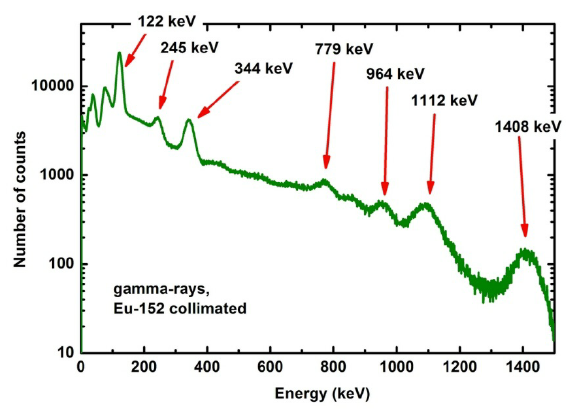
\includegraphics[width=0.50\textwidth]{espectro_de_referencia.png}
  \caption{Espectro de referencia del Eu-152.}
  \label{fig:eu152_ref}
\end{figure}


El primer paso en la calibración energética implica visualizar los datos adquiridos. Creamos un gráfico de canal vs. conteos utilizando los datos obtenidos del espectro de $^{152}$Eu. Este gráfico proporciona una representación directa de la distribución de la señal a través de los canales del detector.  Posteriormente, comparamos este gráfico generado con el espectro de referencia representado en la Figura \ref{fig:eu152_ref}. Construimos una tabla que liste sistemáticamente los canales correspondientes a los conteos máximos de cada pico de energía observado en la Figura \ref{eu152_ref}. A continuación, realizamos un análisis de correlación lineal sobre los datos tabulados en la tabla construida anteriormente. Finalmente, reproducimos el gráfico del espectro de $^{152}$Eu, pero esta vez mostrando la energía en el eje x y los conteos en el eje y, permitiendo una visualización directa de la forma espectral en el espacio de energía.

\subsection*{Energía del Pico del $^{137}$Cs}


\begin{figure}[]
  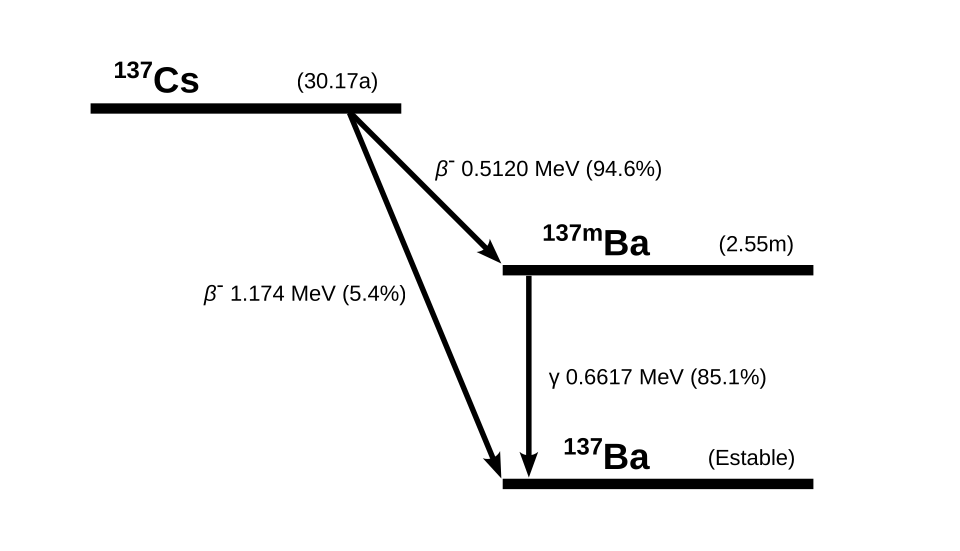
\includegraphics[width=0.50\textwidth]{decaimiento_cesio.png}
  \caption{Decaimiento del Cesio \cite{FirestoneShirley1996} \cite{Garrett1980}.}
  \label{fig:decaimiento_cs}
\end{figure}

Una vez establecida la calibración de la energía, procedemos a analizar el espectro de $^{137}$Cs. Generamos un gráfico de energía vs. conteos utilizando los datos del espectro de $^{137}$Cs, aplicando la calibración determinada previamente. Después de crear el gráfico, identificamos el pico correspondiente a la señal de $^{137}$Cs. Determinamos con precisión el valor de energía en el punto máximo del pico. Verificamos que esta energía medida coincida estrechamente con la energía conocida del fotón gamma emitido por $^{137}$Cs como se describe en la Figura \ref{fig:decaimiento_cs}. Para evaluar el rendimiento del sistema de detección de radiación ionizante, calculamos el Ancho Total a Media Altura (FWHM). El FWHM, una medida estándar de la resolución del detector, representa el ancho del pico a la mitad de su altura máxima y se especifica típicamente a una energía dada. Calculamos el FWHM para el pico de $^{137}$Cs para cuantificar la capacidad del detector para resolver características espectrales estrechamente espaciadas.

\section{Resultados y discusión}

\begin{figure}[]
  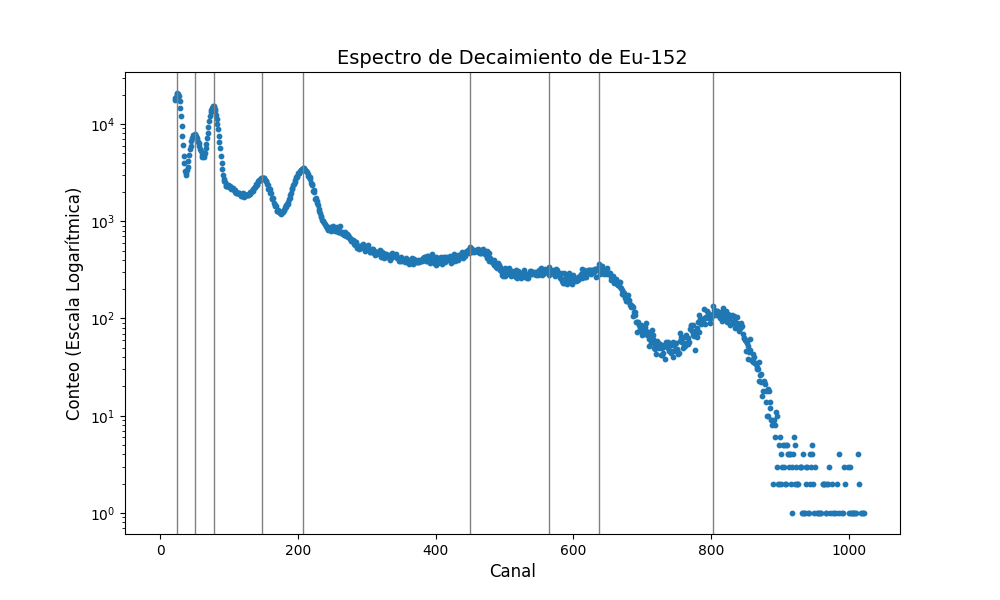
\includegraphics[width=0.50\textwidth]{Eu-152_graph.png}
  \caption{Gráfico del espectro de Eu-152.}
  \label{fig:eu152_graph}
\end{figure}

\subsection*{Calibración de la Energía}
Para calibrar la energía comenzamos por graficar el conteo (en una escala logarítmica) contra el canal de los datos proporcionados para el Eu-152. Encontramos los máximos segmentando los datos en de manera que cada segmento contenga sólo un máximo y luego simplemente tomando función máximo de python, proceso que implementamos en la función find\_local\_maxima del archivo rayos\_gamma/calibrar\_energia.py del repositorio del laboratorio \cite{BrianDL_laboratorio}. El resultado se puede ver en la figura \ref{fig:eu152_graph}.

Luego procedemos a comparar los máximos encontrados con la figura proporcionada \ref{fig:eu152_ref}, lo cual nos permite construir la tabla \ref{tab:channels_energies} que relaciona el canal con su energía respectiva.

\begin{table}[h]
  \centering
  \begin{tabular}{c c}
      \hline
      Canal & Energía (KeV) \\
      \hline
      78 & 122 \\
      148 & 245 \\
      207 & 344 \\
      450 & 779 \\
      564 & 964 \\
      637 & 1112 \\
      802 & 1408 \\
      \hline
  \end{tabular}
  \caption{Canales y sus energías correspondientes.}
  \label{tab:channels_energies}
\end{table}

Luego procedimos a realizar un encaje lineal entre la energía y el canal correspondiente de acuerdo a la ecuación $E = mc +b$ el cual nos permite encontrar la relación entre ambas variables. El encaje se realiza en el script rayos\_gamma/encaje\_energia.py, el cual nos produce también la figura \ref{fig:energia_canal_graph} donde podemos apreciar también la línea de encaje y los respectivos valores para $m = 1.77$ y $b = -19.73$.

\begin{figure}[]
  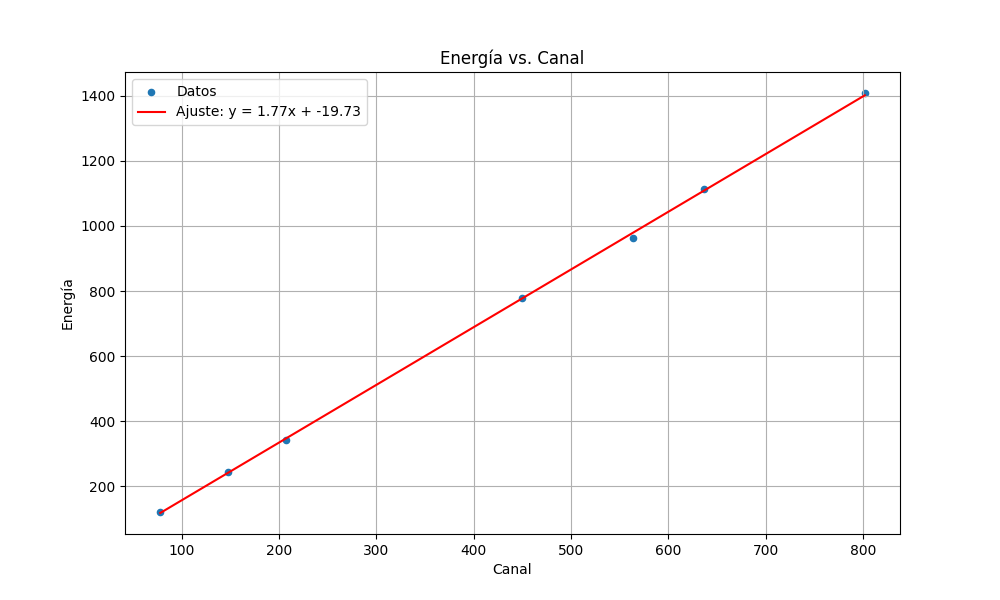
\includegraphics[width=0.50\textwidth]{energy_vs_canal.png}
  \caption{Energía contra canal de datos.}
  \label{fig:energia_canal_graph}
\end{figure}

Utilizando estos resultados podemos obtener ahora el gráfico del conteo sobre la energía, como se muestra en la figura \ref{fig:energia_conteo_graph} 

\begin{figure}[]
  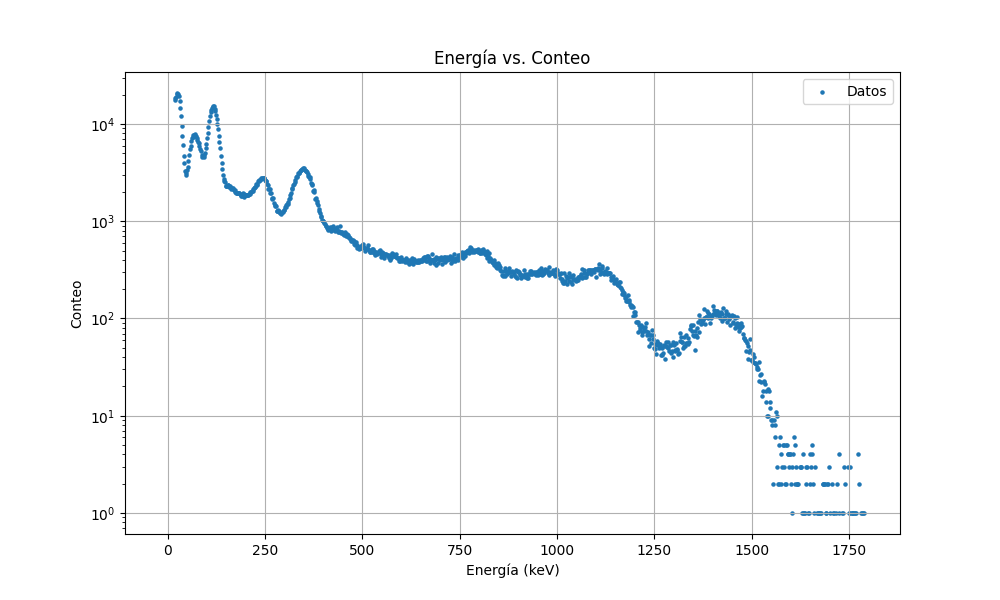
\includegraphics[width=0.50\textwidth]{energia_vs_conteo_eu-152.png}
  \caption{Energía contra conteo.}
  \label{fig:energia_conteo_graph}
\end{figure}

\subsection*{Energía del Pico de $^{137}Cs$}

\begin{figure}[h]
  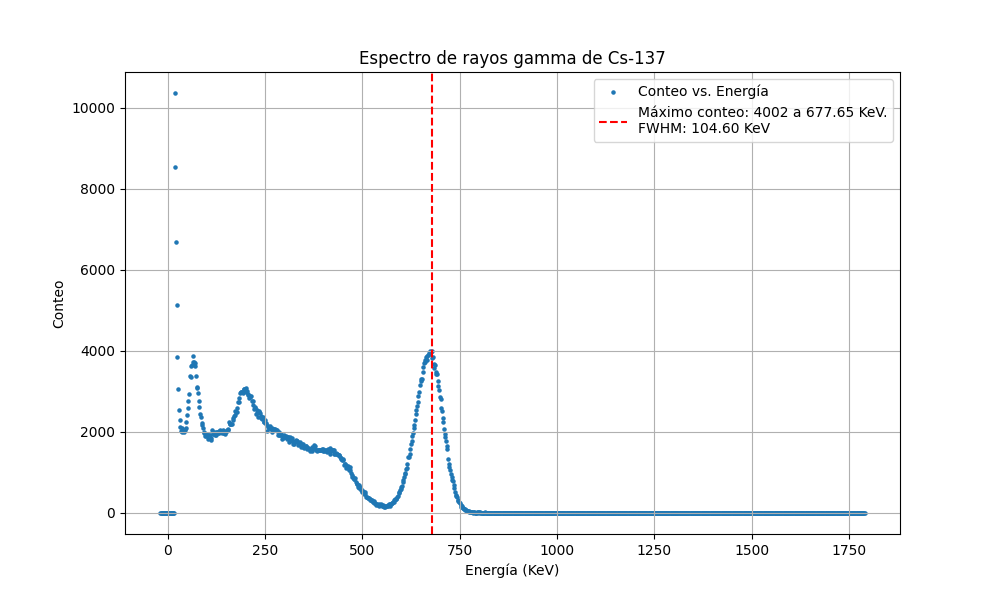
\includegraphics[width=0.50\textwidth]{plot_cs137.png}
  \caption{Espectro del $^{137}Cs$.}
  \label{fig:espectro_cs}
\end{figure}

Los valores encontrados para $m, b$ nos permiten también encontrar el máximo de energía para el espectro del $^{137}Cs$. El cual procedemos a graficar en la figura \ref{fig:espectro_cs}. Donde podemos observar el máximo encontrado para la energía $E= 0.678$ MeV. Lo cual concuerda bastante bien con el valor esperado de 0.66 MeV \ref{fig:decaimiento_cs}.
Para encontrar el máximo conteo según la energía procedimos a tomar la función max de python después de filtrar las energías y tomar sólo el rango (550,750), los cuales visualmente podemos verificar que contienen sólo el máximo que nos interesa.
La figura \ref{fig:espectro_cs} también nos muestra nuestro cálculo de fwhm = 104.6 KeV \cite{Martin2010} el cual calculamos realizando un encaje cuadrático a los datos en la región de energías mencionadas (550,750) y luego restando la distancia entre los dos intersectos de este encaje con la recta horizontal a media altura del máximo. El código para calcular el máximo, el fwhm y graficarlos se encuentra en graficar\_conteo\_vs\_energia\_cs.py

\section{Conclusiones}

Se logró la calibración del sistema de medición de energía, estableciendo una relación lineal entre el canal de conteo y la energía depositada por los rayos gamma. Esta calibración permitió convertir las lecturas del detector en valores de energía precisos.

También se observó la característica forma espectral de la desintegración de Cs-137, caracterizada por un pico prominente a aproximadamente 662 keV.  El cálculo del Ancho a Media Altura (FWHM) del pico resultó en un valor de 104.6 KeV.

\bibliographystyle{ieeetr}
\bibliography{referencias} 

\end{document}